\documentclass[11pt]{extarticle}

% meta
\title{Отчет о лабораторной работе №2 \\[6mm] \large Обработка и распознавание изображений, ММП ВМК МГУ.}
\author{Аристархов Данила Дмитриевич.}
\date{Март 2024.}

\usepackage[warn]{mathtext}
\usepackage[T2A]{fontenc}			% кодировка
\usepackage[utf8]{inputenc}			% кодировка исходного текста
\usepackage[english,russian]{babel}	% локализация и переносы
\usepackage{indentfirst}
\usepackage{csquotes}
\usepackage{svg}
\usepackage{wrapfig}
\usepackage{listings}
% \usepackage[bibstyle=gost-numeric, sorting=none]{biblatex}
% \addbibresource{biblio.bib}

% page settings
\usepackage[
    left=1.8cm,
    right=1.8cm,
    top=1.8cm,
    bottom=1.8cm,
    bindingoffset=0cm
]{geometry}

\usepackage{graphicx, hyperref, xcolor}
\hypersetup{
    colorlinks=true,
    linkcolor=blue,
    filecolor=magenta, 
    urlcolor=blue,
    citecolor=blue,
    pdftitle={GD},
    % pdfpagemode=FullScreen,
    linktoc=all
    }

\usepackage{wrapfig,caption}

% figures
\usepackage{caption}
\usepackage{subcaption}
\usepackage{floatrow}
\floatsetup{heightadjust=object}

\graphicspath{{img}}

% math
\usepackage{amsmath,amsfonts,amssymb,amsthm,mathtools,esint,eucal}

\begin{document}

\maketitle
{
  \hypersetup{linkcolor=black}
  \tableofcontents
}
\newpage

\section{Постановка задачи}
Необходимо разработать и реализовать программу для работы с изображениями фишек игрового набора Тримино. Программа должна производить сегментацию изображения, а также подсчет количества точек на фишках. Также необходимо разработать пользовательский интерфейс для работы с программой, обеспечивающий выбор изображения, выполнение операций преобразования и выдачу результата.

\section{Описание данных}
Данные представляют из себя растровые изображения, на которых изображены фишки Тримино на различных фонах. Фишки представляют из себя треугольники с нанесенными на 3 углах точками. Количество точек варьируется от 0 до 5.

\begin{figure}[h]
  \centering
  \includesvg[width=\textwidth]{Segmentate}
  \caption{Пример работы модели сегментации}
  \label{fig:segmentate}
\end{figure}

\section{Описание метода решения}
\subsection{Сегментация изображения}

\begin{wrapfigure}{r}{0.5\textwidth}
  \centering
  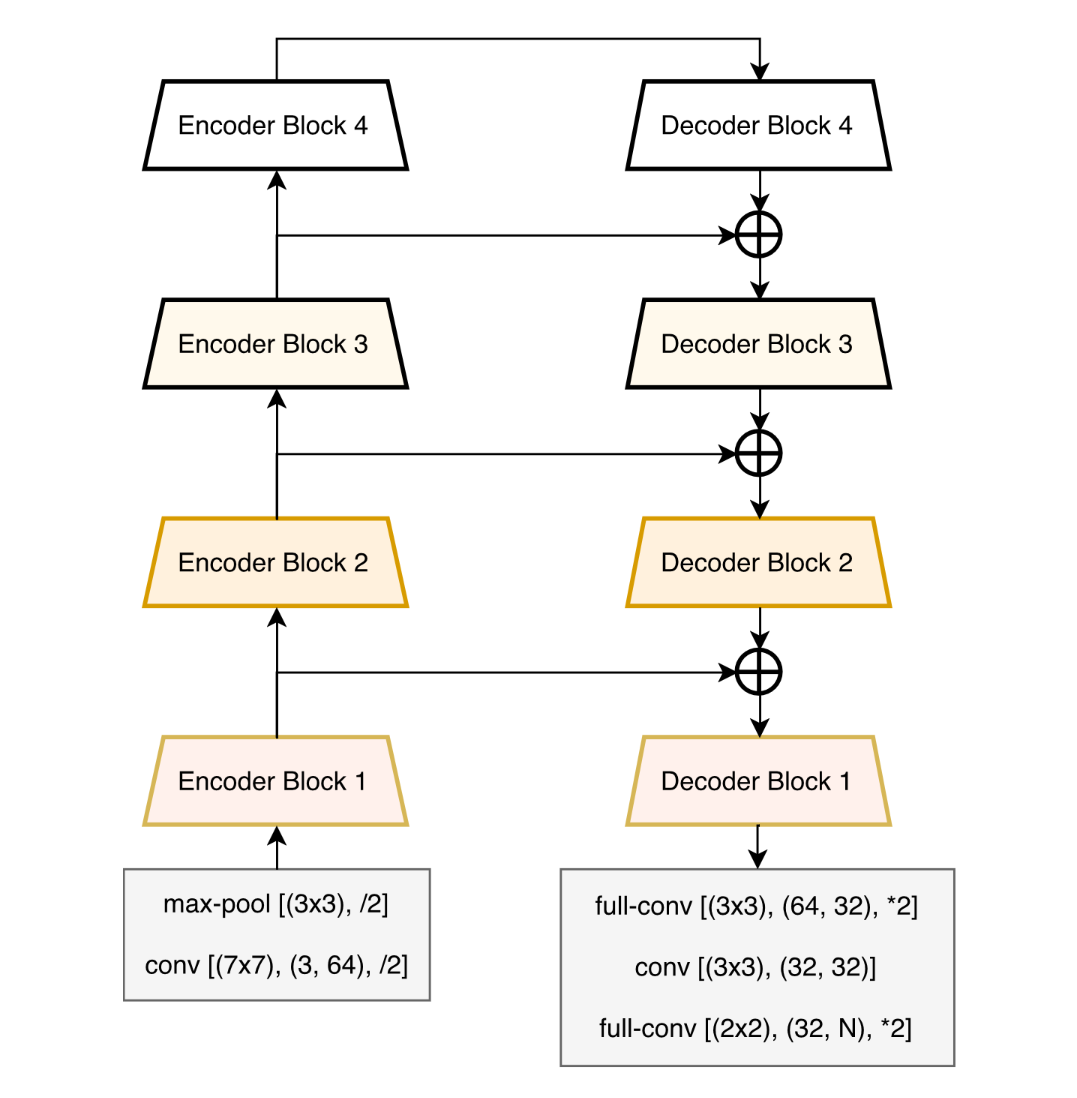
\includegraphics[width=\textwidth]{LinkNet}
  \caption{Архитектура LinkNet}
  \label{fig:linknet}
\end{wrapfigure}

Для сегментации изображений был применен нейросетевой подоход. Для этого изображения предварительно были размечены вручную. В качестве архитектуры была выбрана LinkNet (\autoref{fig:linknet}) с использованием энкодера, основанного на VGG13. Обучение производилось c помощью различных аугментаций, таких как вырезание случайного фрагмента изображения, горизонтальное отражение, изменение яркости и т.д. 

Для улучшения результата работы модели при постобработке были использованы следующие морфологический операции:
\begin{enumerate}
  \item Закрытие с ядром $(13, 13)$ для устранения полостей в полученной маске сегментации.
  \item Эрозия с ядром $(13, 13)$ для разъединения на отдельные компоненты близко расположенных треугольников и удаления шума. Также это преобразование позволяет отделиться от границы треугольника, что поможет на этапе подсчета точек.
\end{enumerate}

\subsection{Поиск фишек}
Для поиска отдельных фишек сначала выделялись границы полученной маски. Затем эти границы приближались многоугольниками. Из этих многоугольнов выбирались треугольники. Таким образом удается выделить вершины фишек, и с помощью этого вычислить центр фишки.

\subsection{Подсчет точек}
Подсчет точек происходит в несколько этапов:
\begin{enumerate}
  \item Считается градиент изображения по горизонтали $G_x$ и по вертикали $G_y$ отдельно по цветовым каналам.
  \item Вычисляется общий градиент $G = |G_x| + |G_y|$.
  \item Получаем маску с помощью максимума градиента по каналам.
  \item Эта маска размывается по Гауссу с ядром размера $(3, 3)$.
  \item Производится бинаризация Оцу полученной маски.
  \item Для каждой вершины треугольников берется ее окрестность. Эта окрестность представляет из себя пересечение маски треугольника, полученной при сегментации, и окружности с радиусом, равным расстоянию от вершины до центра треугольника.
  \item В этой окрестости ищется количество связных компонент. При этом происходит отсев слишком маленьких компонент.
\end{enumerate}
Число связных компонент и является количеством точек возле вершины фишки.


\begin{figure}[h]
  \centering
  \begin{subfigure}[b]{0.3\textwidth}
    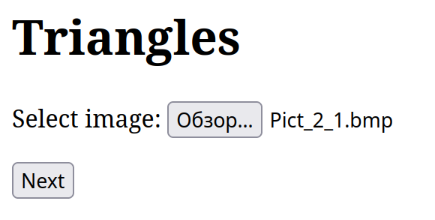
\includegraphics[width=\textwidth]{server1}
    \caption{Выбор изображения}
  \end{subfigure}
  \begin{subfigure}[b]{0.7\textwidth}
    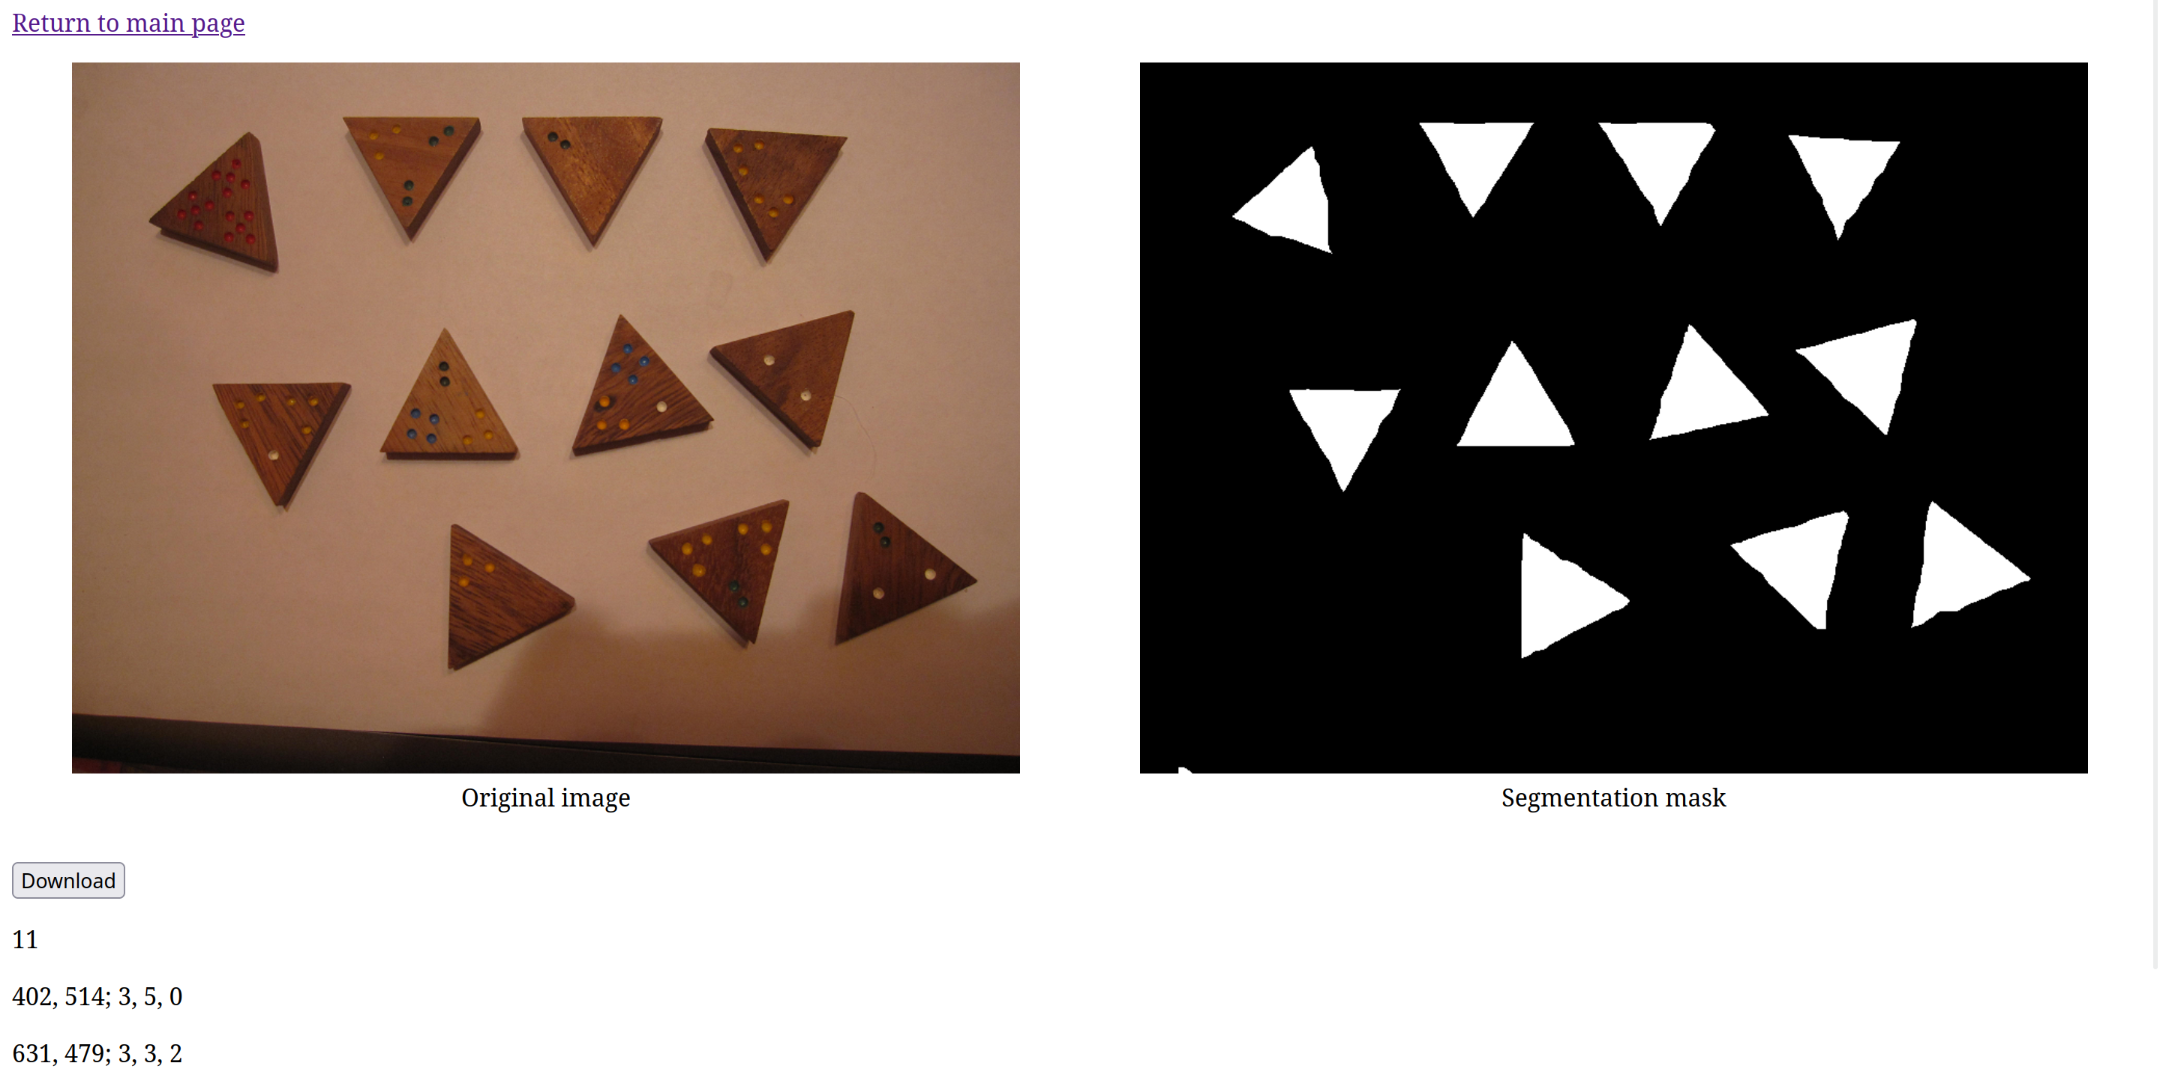
\includegraphics[width=\textwidth]{server2}
    \caption{Результат работы программы}
  \end{subfigure}
  \caption{Этапы работы с программой}
  \label{fig:program}
\end{figure}

\section{Описание программой реализации}
Программа была написана на языке программирования \verb|Python|. Для работы с изображениями использовалась библиотека \verb|OpenCV|. Для обучение нейросети был использована библиотека \verb|PyTorch|, для аугментаций --- \verb|Albumentations|. Интерфейс был реализован в виде веб-сервера с помощью библиотеки \verb|Flask|. Для удобство решение было обернуто в docker-контейнер, однако возможна установка программы и всех зависимостей вручную.

Работа с программой происходит следующим образом (см. \autoref{fig:program}): сначала пользователь выбирает изображение для обработки.
Далее происходит выдача результата в виде маски сегментации исходного изображения, а также координаты центров фишек и результат подсчета количества точек в углах. Имеется возможность скачать результат в виде файла формата \verb|txt|.


\section{Эксперименты}

\begin{figure}[h]
  \centering
  \begin{subfigure}[b]{0.45\textwidth}
    \includesvg[width=\textwidth]{exp1}
    \caption{Beginner}
  \end{subfigure}
  \begin{subfigure}[b]{0.45\textwidth}
    \includesvg[width=\textwidth]{exp2}
    \caption{Expert}
  \end{subfigure}
  \caption{Эксперименты}
  \label{fig:exp}
\end{figure}

Алгоритм отлично себя показал на этапе сегментации исходного изображения. Хотя нейросеть хорошо выделяет фишки на любом фоне при любом освещении. С помощью морфологии удается устранить различные неточности нейросети: убрать шум, отделить треугольники друг от друга и заполнить полости внутри них. Также выделение только треугольных компонент позволяет убрать лишние компоненты и получить координаты вершин треугольника.

Алгоритм подсчета точек тоже хорошо справился с задачей. Однако на некоторых иногда результаты получаются неточными. В первую очередь это происходит из-за неоднородности фишки, что влечет появление градиента на фишки не в местах расположения точек. Также алгоритм имеет трудности с классификацией 5 точек, поскольку они плотно расположены и их трудно отделить друг от друга. Возможным решением данной проблемы является фотографирование фишек более крупным планом.

\section{Выводы}
Предложенный алгоритм смог добиться высокой точности при сегментации изображения. Классификация фишек происзодит менее точно, однако выдает результат, близкий к реальному количеству точек. В целом алгоритм смог справиться с поставленной задачей

\end{document}